\section{Solvers for SDEs}
Considering now the stochastic differential equation (SDE)
$$
d x(t)=f\left(t, x(t), p_{f}\right) d t+g\left(t, x(t), p_{g}\right) d \omega(t) \quad d \omega(t) \sim N_{i i d}(0, I \Delta t)
$$

where $x \in \mathbb{R}^{n_{x}}$ and $\omega$ is a multivariate stochastic variable following a Wiener Process. The first term \textit{f()} is commonly referred to as the \textit{drift term} and the ladder term \textit{g()} is commonly referred to as the \textit{diffusion term}. The ODE is a particular case of an SDE where $g() = 0$. If the diffusion $g()$ does not change for different values of $x(t)$ the diffusion is said to be \textit{state independent} and said to be \textit{state dependent} otherwise.

\subsection{Wiener Process}
The Wiener Process is a stochastic process (a sequence of stochastic variables) realised from identical and independent Gaussian distributions with 0 mean and variance increasing with time \textit{dt}. It therefore models continuous perturbations allowing for greater variation when more time has passed. Using the reparametrization trick one can pull out the variance and use the standard Gaussian. It is implemented in MATLAB as follows:

\begin{adjustwidth*}{0cm}{-0.4cm}
\begin{lstlisting}[frame=single, language=Matlab,caption=Wiener Process, label=LittleWiener]
function [W,Tw,dW] = StdWienerProcess(T,N,nW,Ns,seed)
if nargin == 4
    rng(seed);
end
dt = T/N; % Fixed step size
dW = sqrt(dt)*randn(nW,N,Ns);
W = [zeros(nW,1,Ns) cumsum(dW,2)];
Tw = 0:dt:T;
\end{lstlisting}
\end{adjustwidth*}

\subsection{Explicit-Explicit (Euler-Maruyama)}
An SDE solver has to address both the drift term and the diffusion term. By linearity of integration the integral can be split into two integrals

\begin{equation}
\boldsymbol{x}\left(t_{k+1}\right)-\boldsymbol{x}\left(t_{k}\right)=\int_{t_{k}}^{t_{k+1}} f(\boldsymbol{x}(t)) d t+\int_{t_{k}}^{t_{k+1}} g(\boldsymbol{x}(t)) d \boldsymbol{\omega}(t)
\end{equation}

The drift term can be solved by a Riemann integral for which we have numerous approximation methods normally associated with ODEs. The diffusion term however requires an Itô integral \cite{JrgensenScientificEquationsd}. "Explicit-Explicit" refers to solving the drift term with an explicit method and the diffusion term with an explicit method. We will use the Euler-Maruyama for approximating the solution to the SDE:

\begin{equation}
\boldsymbol{x}_{k+1}-\boldsymbol{x}_{k}=f\left(\boldsymbol{x}_{k}\right) \Delta t_{k}+g\left(\boldsymbol{x}_{k}\right) \Delta \boldsymbol{w}_{k}
\end{equation}

Where we will use a fixed step size $\Delta t_k = \Delta t$. Note how the SDE is discretized as usual. It is based on a forward step $f\left(\boldsymbol{x}_{k}\right)$ for the drift and a forward step $g\left(\boldsymbol{x}_{k}\right)$ for the diffusion, i.e. Explicit-Explicit. The MATLAB implementation is found below.

\begin{adjustwidth*}{0cm}{-0.4cm}
\begin{lstlisting}[frame=single, language=Matlab,caption=Euler-Maruyama, label=hnrkmdsen]
function X = SDEsolverExplicitExplicit(ffun,gfun,T,x0,W,varargin)
N = length(T);
nx = length(x0);
X = zeros(nx,N);

X(:,1) = x0;
for k=1:N-1
    f = feval(ffun,T(k),X(:,k),varargin{:});
    g = feval(gfun,T(k),X(:,k),varargin{:});
    dt = T(k+1)-T(k); % Allow for varying step size
    dW = W(:,k+1)-W(:,k);
    psi = X(:,k) + g*dW; % The diffusion/pertubation 
    X(:,k+1) = psi + f*dt; % Add the drift
end
\end{lstlisting}
\end{adjustwidth*}

\subsection{Implicit-Explicit}
Now the drift term can also be solved by an Implicit Euler method as shown in Section 3. The approximation to the SDE is then

\begin{equation}
\boldsymbol{x}_{k+1}=\boldsymbol{x}_{k}+f\left(\boldsymbol{x}_{k+1}\right) \Delta t_{k}+g\left(\boldsymbol{x}_{k}\right) \Delta \boldsymbol{w}_{k}
\end{equation}

Where we will use a fixed step size $\Delta t_k = \Delta t$. Note how it is based on $f\left(\boldsymbol{x}_{k+1}\right)$ for the drift, where $x_{k+1}$ is unknown and calculated implicitly. The step for the diffusion is an explicit forward step $g\left(\boldsymbol{x}_{k}\right)$ for the diffusion. In other words, the method is an Implicit-Explicit method. The MATLAB implementation is found below.

\begin{adjustwidth*}{0cm}{-0.4cm}
\begin{lstlisting}[frame=single, language=Matlab,caption=Implicit-Explicit, label=implicitexplicit]
function X=SDEsolverImplicitExplicit(ffun,gfun,T,x0,W,tol,varargin)
maxit = 100;

N = length(T);
nx = length(x0);
X = zeros(nx,N);

X(:,1) = x0;
k=1;
[f,~] = feval(ffun,T(k),X(:,k),varargin{:});
for k=1:N-1
    g = feval(gfun,T(k),X(:,k),varargin{:});
    dt = T(k+1)-T(k);
    dW = W(:,k+1)-W(:,k);
    psi = X(:,k) + g*dW;
    xinit = psi + f*dt;
    [X(:,k+1),f,~] = SDENewtonSolver(...
            ffun,...
            T(:,k+1),dt,psi,xinit,...
            tol,maxit,varargin{:});
end
\end{lstlisting}
\end{adjustwidth*}

As with the Implicit Euler in Section 3, it is based on Newton's method for finding a root of the residual function by iteratively taking steps along the Jacobian evaluated in the current iteration. The implementation is seen in Listing \ref{newtonsde}.

\begin{adjustwidth*}{0cm}{-0.4cm}
\begin{lstlisting}[frame=single, language=Matlab,caption=Newton's Method for SDEs, label=newtonsde]
function [x,f,J] = SDENewtonSolver(ffun,t,dt,psi,xinit,tol,maxit,varargin)
I = eye(length(xinit));
x = xinit;
[f,J] = feval(ffun,t,x,varargin{:});
R = x - f*dt - psi;

it=1;
while( (norm(R,'inf') > tol) && (it <= maxit) )
    dRdx = I - J*dt;
    mdx = dRdx\R;
    x = x - mdx;
    [f,J] = feval(ffun,t,x,varargin{:});
    R = x - f*dt - psi;
    it = it+1;
end
\end{lstlisting}
\end{adjustwidth*}


\subsection{Description of implementations}
Implementations and methods has already been described and code included under the relevant methods in Section 4.2 and 4.3.

\subsection{Van der Pol}
In this section the above listed MATLAB implementations are tested on the Van der Pol problem. Until now we have only modelled a deterministic drift. The Van der Pol problem is now extended with a diffusion term. Two different diffusion functions will be tested, a state independent and state dependent respectively:

\begin{align*}
    & g(t, \boldsymbol{x}(t), \sigma) = [0, \sigma]^T \quad (1) \\
    & g(t, \boldsymbol{x}(t), \sigma) = [0, \sigma (1 + x_1(t)^2)]^T \quad (2)
\end{align*}

Resulting in SDE version (1) of the Van der Pol problem:

\begin{equation}
\label{sde1}
\begin{aligned}
d x_{1}(t) &=x_{2}(t) d t \\
d x_{2}(t) &=\left[\mu\left(1-x_{1}(t)^{2}\right) x_{2}(t)-x_{1}(t)\right] d t+\sigma d \omega(t)
\end{aligned}
\end{equation}

And SDE version (2) of the Van der Pol problem:

\begin{equation}
\label{sde1}
\begin{aligned}
&d x_{1}(t)=x_{2}(t) d t \\
&d x_{2}(t)=\left[\mu\left(1-x_{1}(t)^{2}\right) x_{2}(t)-x_{1}(t)\right] d t+\sigma\left(1+x_{1}(t)^{2}\right) d \omega(t)
\end{aligned}
\end{equation}

And fixed step size of $\Delta t = h = 0.001$ is used.







\\\

\textbf{Version (1) - state independent diffusion}
In this section, equation (\ref{sde1}) is solved for realizations with $\sigma \in \{0.1 2.0\}$:

\begin{figure}
    \centering
    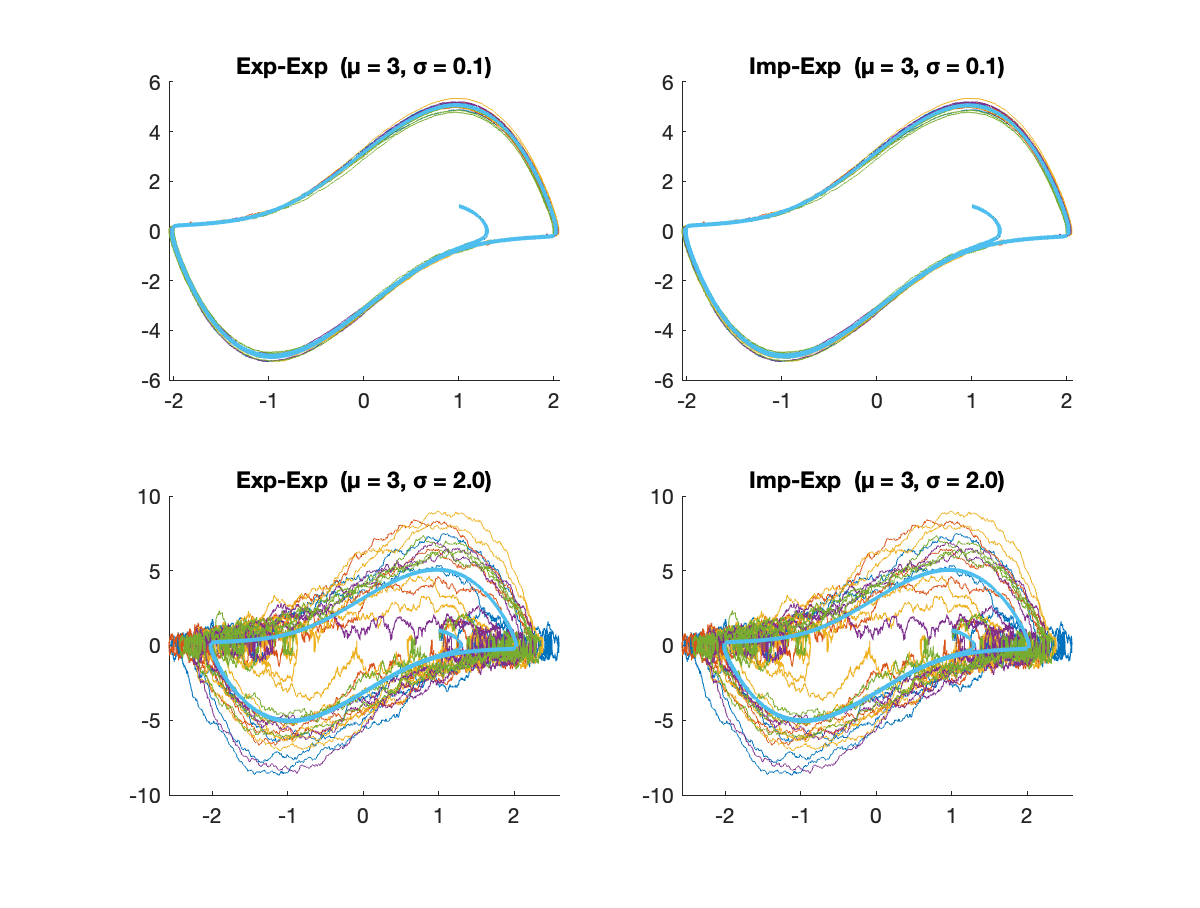
\includegraphics[width=\textwidth]{plots/4b.eps}
    \caption{cap}
    \label{fig:4b}
\end{figure}

\begin{figure}
    \centering
    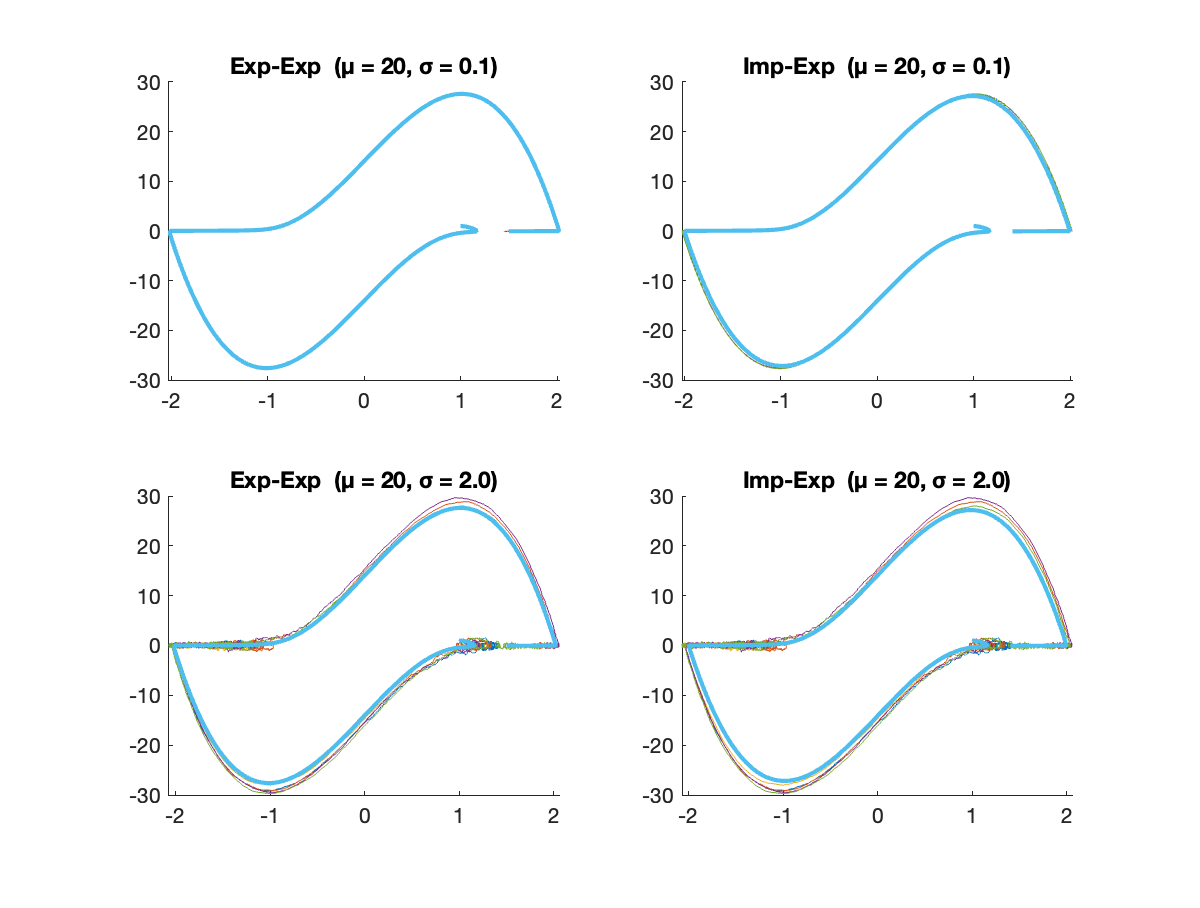
\includegraphics[width=\textwidth]{plots/4a.eps}
    \caption{cap}
    \label{fig:4a}
\end{figure}

\textbf{Version (1) - state independent diffusion}
In this section, equation (\ref{sde1}) is solved for realizations with $\sigma \in \{0.1 2.0\}$:

\begin{figure}
    \centering
    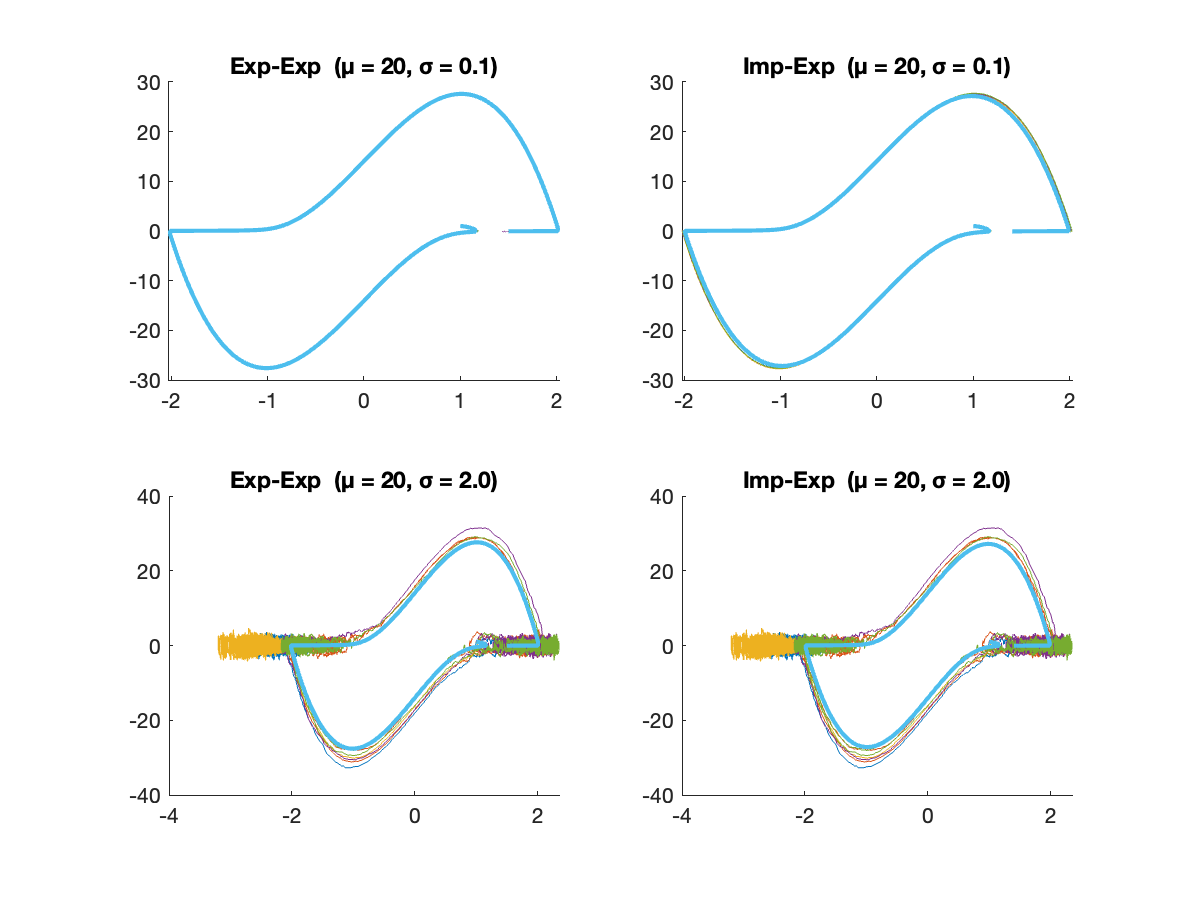
\includegraphics[width=\textwidth]{plots/4c.eps}
    \caption{cap}
    \label{fig:4b}
\end{figure}

\begin{figure}
    \centering
    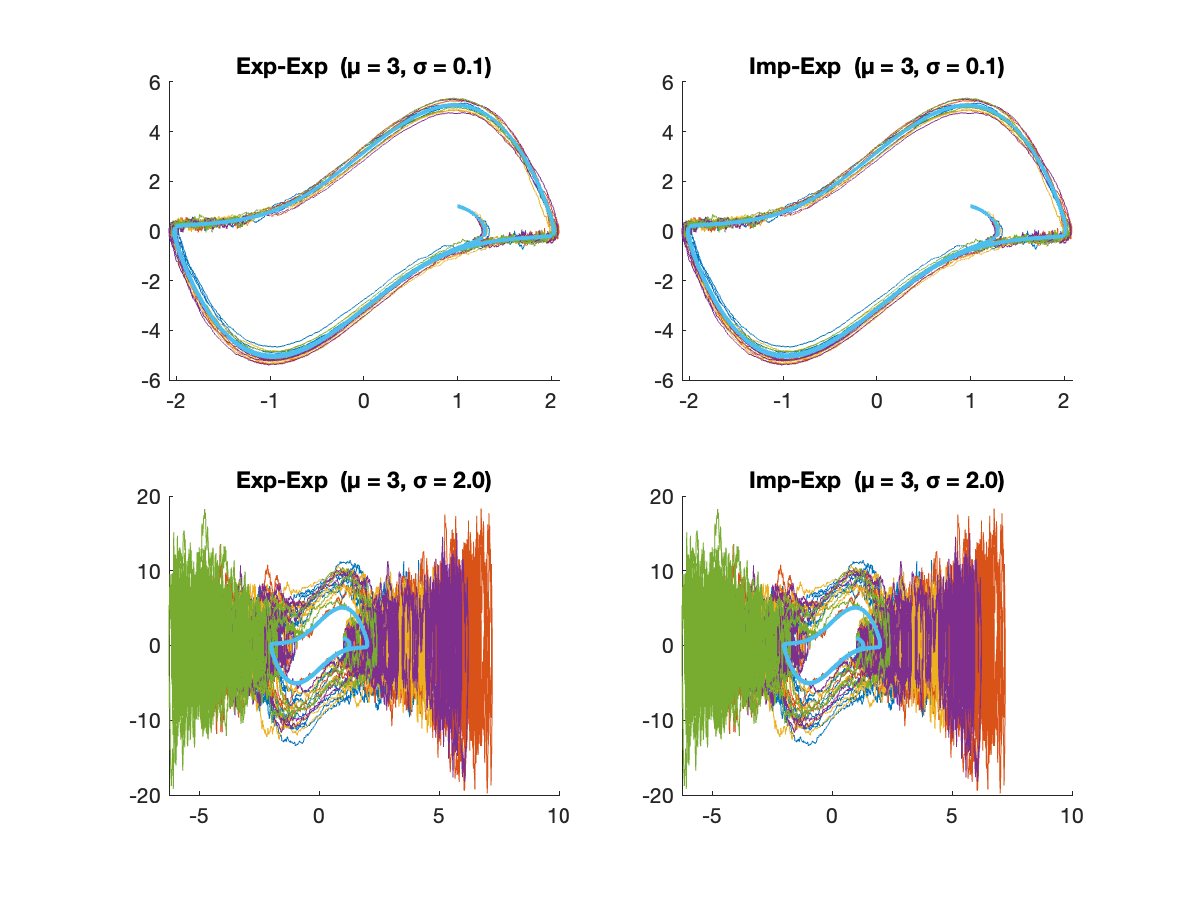
\includegraphics[width=\textwidth]{plots/4d.eps}
    \caption{cap}
    \label{fig:4a}
\end{figure}

